\chapter{Optimizing SteelEagle Performance}

As explained in \cref{sec:overview}, the performance of the SteelEagle system
determines its versatility. A drone that is slow to react will be unable to
effectively navigate obstacle-dense environments. The chances of the drone
losing track of a fast on-ground target that is moving erratically increases
substantially if the drone is slow in keeping the target centered in its view.
Given the importance of performance, this chapter details how performance is
defined for SteelEagle, how it is measured, and work done to identify
performance bottlenecks and optimize the system.

\begin{figure}[htbp]
\centerline{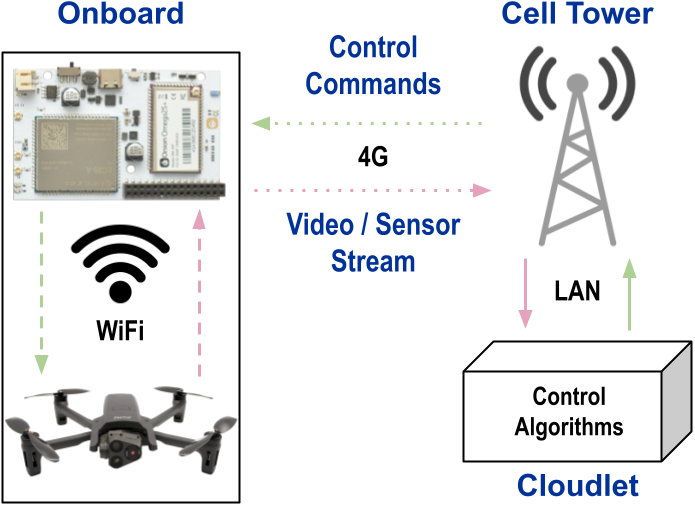
\includegraphics[width = .5\textwidth]{figs/fig-simplified-arch.png}}
\caption{SteelEagle Edge Offload Pipeline}
\label{fig:simplified-arch}
\end{figure}

\section{How is performance defined in SteelEagle?}
\label{sec:steeleagle-performance-def}

The performance of SteelEagle is determined by the end-to-end latency and
throughput of the system. \cref{sec:overview} explained how drones in
SteelEagle are treated as thin clients, with the use of a communications relay
to make up for the lack of cellular connectivity on commerical-off-the-shelf
(COTS) drones. The sensor stream from the drone is forwarded to the
communications relay over Wi-Fi, which in turn forwards it to the cloudlet over
4G LTE. After performing inference on the received data, the cloudlet sends
back piloting commands to the drone, via a hop through the communications relay
(\cref{fig:simplified-arch}). As a result, the end-to-end performance is
determined by several components of the pipeline:
\begin{enumerate}
    \item[(a)] On-drone sensing
    \item[(b)] On-drone pre-processing
    \item[(c)] Tranmission to cloudlet
    \item[(d)] Cloudlet processing
    \item[(e)] Transmission to drone
    \item[(f)] Drone post-processing
    \item[(g)] Drone actuation
\end{enumerate}

Each of these components has a latency associated with it, and a throughput
that it is capable of. The performance of components (a), (b), (f), and (g) is
fixed for a given drone. Factors such as the drone camera's sensor readout time
and shutter speed used affect the frame capture latency, and thus determine the
performance of component (a). Component (b) consists of any processing of the
sensor data before it is transmitted from the drone. The generation of an H.264
stream, for instance, adds latency since the compression process is
computationally intensive, involving analysis of deltas between successive
frames. For components (c) and (e), performance is determined by the cellular
network used for communication between the relay and the cloudlet. While there
is variance associated with the performance of these components, factors such
as the number of network hops, distance between the relay to the cloudlet, and
the network signal strength available to the relay largely determine the mean
value of their latency and throughput over a longer period of time. The
performance of component (d) can vary largely based on whether decoding of the
drone stream data is required and type of inferencing that is performed. A DNN
with a complex architecture, for instance, can take much longer for inference
than a traditional computer vision approach. The same inference can also take
less time on a more powerful edge server.

\begin{figure}[htbp]
\definecolor{observe-color}{RGB}{175,208,149}
\definecolor{orient-color}{RGB}{255, 255, 166}
\definecolor{decide-color}{RGB}{255,170,149}
\definecolor{act-color}{RGB}{224,194,205}
\centering
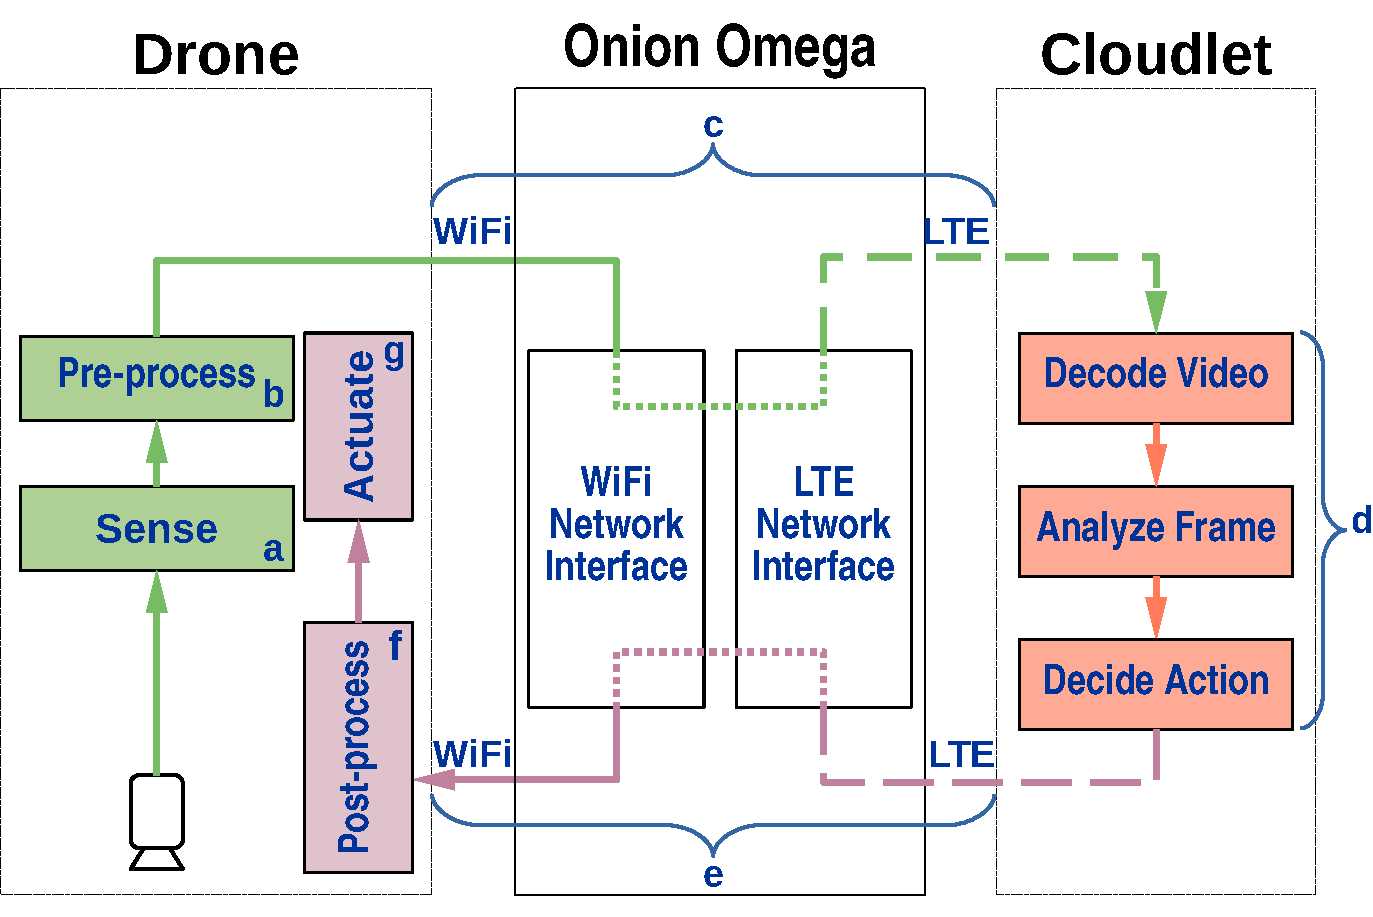
\includegraphics[width = .6\textwidth]{figs/fig-ooda-loop.pdf}\\
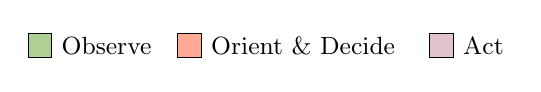
\begin{tikzpicture}
    \draw[fill=observe-color] (1.0,0) rectangle (1.3,0.3);
    \node[right] at (1.3,0.15) {\small Observe};

    \draw[fill=decide-color] (2.9,0) rectangle (3.2,0.3);
    \node[right] at (3.2,0.15) {\small Orient \& Decide};

    \draw[fill=act-color] (6.1,0) rectangle (6.4,0.3);
    \node[right] at (6.4,0.15) {\small Act};
\end{tikzpicture}
\caption{Mapping the SteelEagle pipeline to the OODA loop}
\label{fig:ooda-mapping}
\end{figure}

\Cref{fig:ooda-mapping} shows how these components can be mapped to the various
stage of the OODA pipeline. The ``Observe'' phase includes components (a), (b),
and (c). Components (d) maps to the ``Orient'' and ``Decide'' phases. Finally,
components (e), (f), and (g) correspond to the ``Act'' phase.

\begin{figure}[htbp]
\centerline{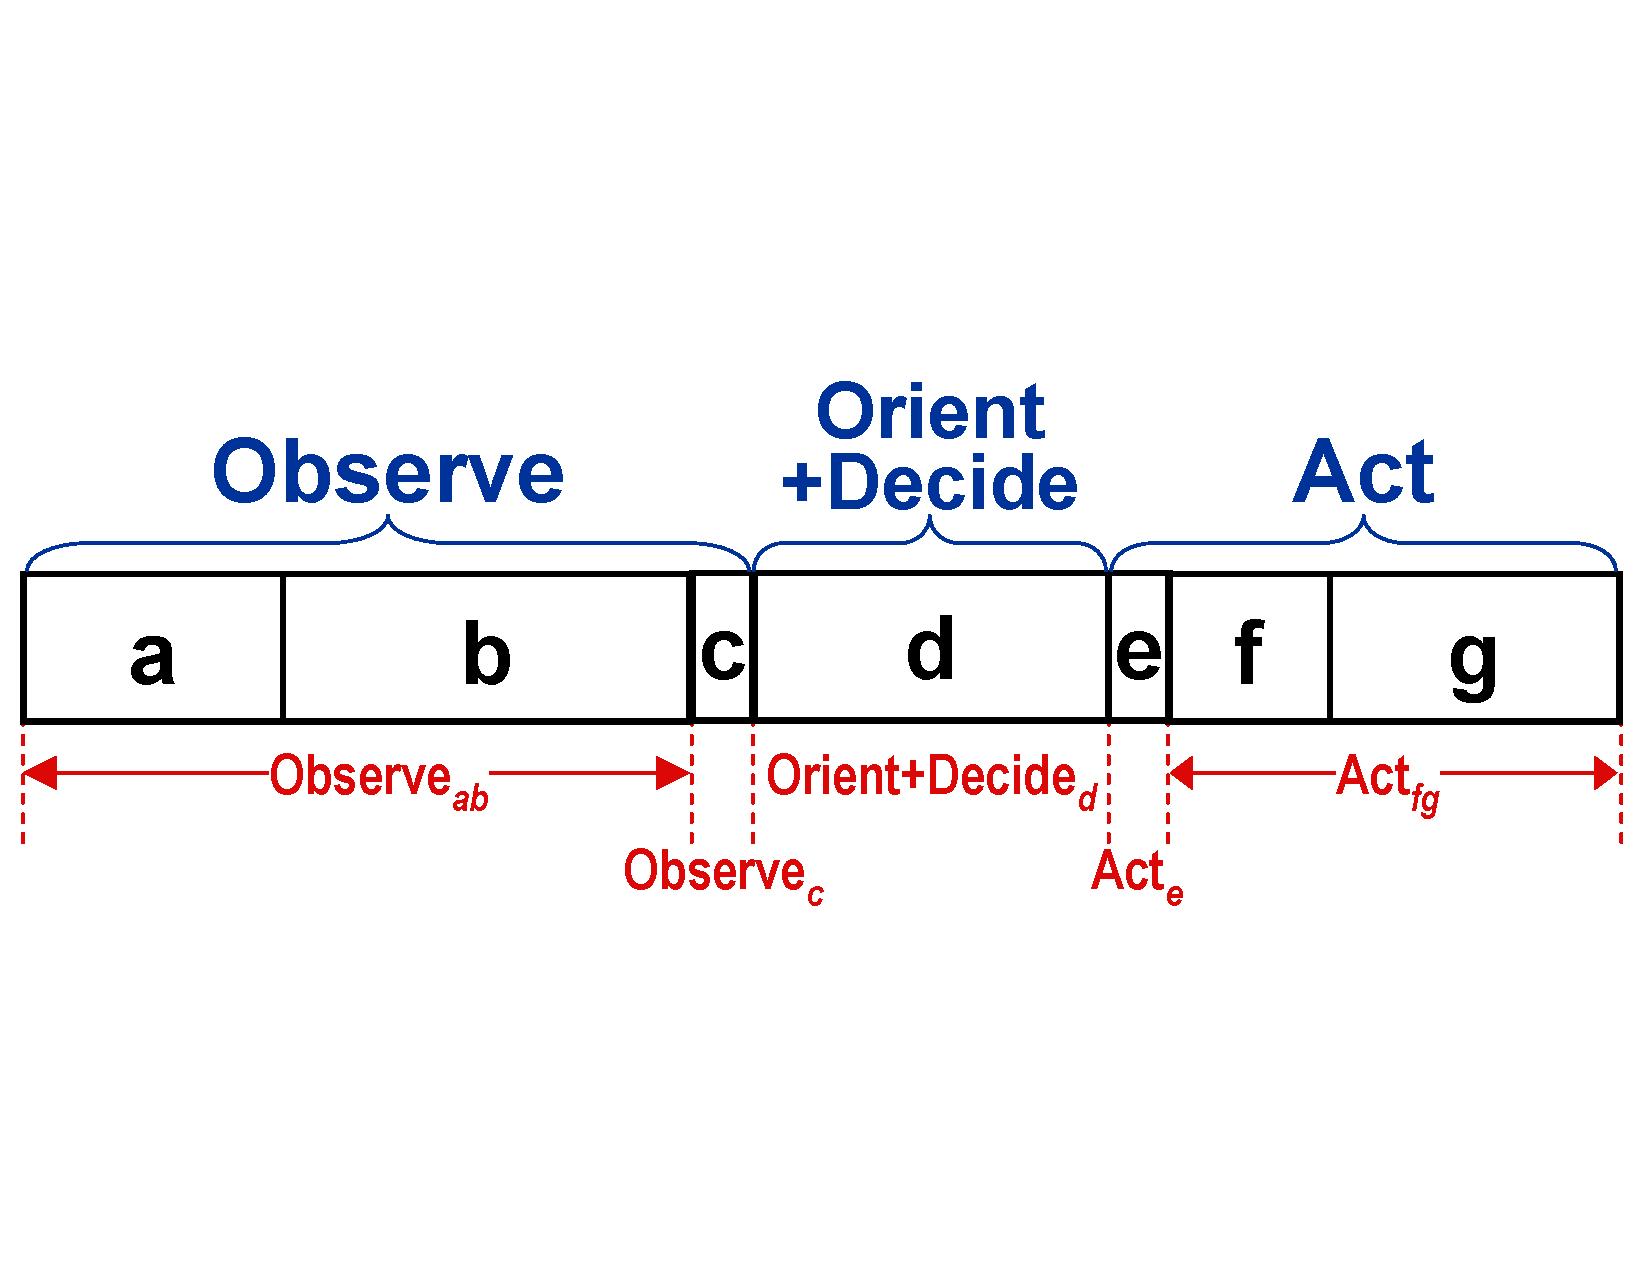
\includegraphics[width = .5\textwidth]{figs/fig-ooda-nomenclature.pdf}}
\caption{Measurable Components of the OODA Loop}
\label{fig:ooda-nomenclature}
\end{figure}

We are limited in our ability to individually measure the contribution of
components of the OODA loop. The drone sensing and pre-processing, components
(a) and (b), for instance, cannot be measured individually because the drone
runs closed source software that does not allow the ability to insert software
instrumentation. Similarly, drone post-processing and actuation must be
measured together.  \Cref{fig:ooda-nomenclature} shows the parts of the
pipeline that can be measured in red.

\section{Measuring the performance of the SteelEagle pipeline}
\label{sec:steeleagle-performance-measurement}

\begin{figure}[htbp]
\centerline{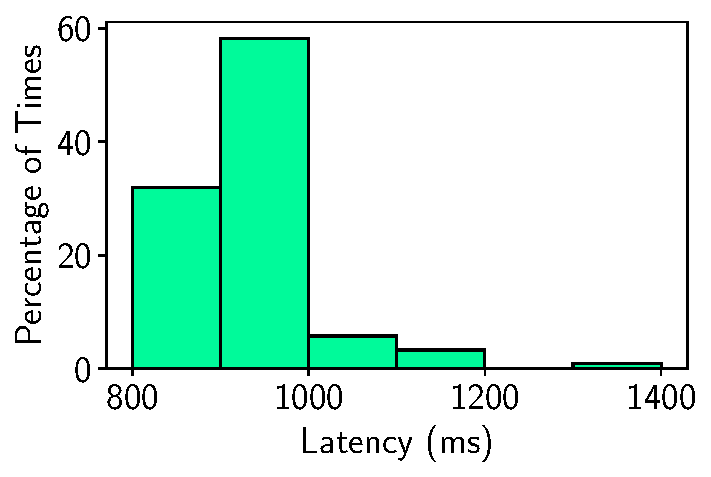
\includegraphics[width = .4\textwidth]{figs/bala_latency.pdf}}
\caption{Original SteelEagle Latency \cite{bala2024}}
\label{fig:steeleagle-original-latency}
\end{figure}

\begin{wrapfigure}{r}{0.25\textwidth}
    \centering
    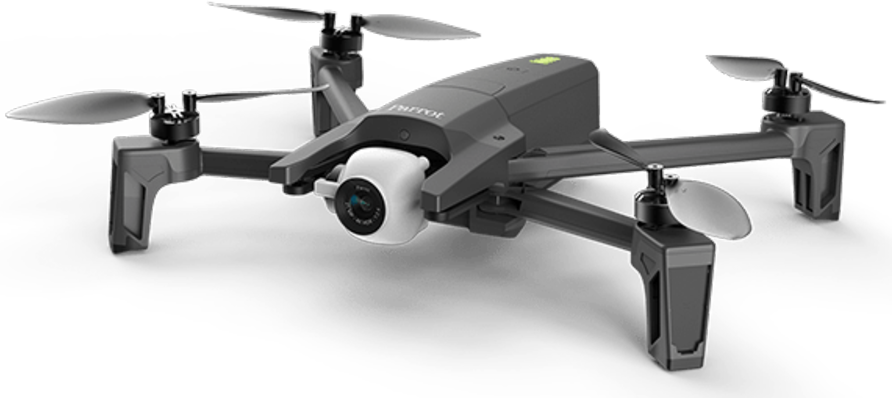
\includegraphics[width=0.2\textwidth]{figs/parrot-anafi.pdf}
    \caption{Parrot Anafi}
    \label{fig:parrot-anafi}
\end{wrapfigure}
The starting point of our investigation into the performance of the SteelEagle
system is the mean drone-to-cloudlet latency of 933 ms reported by Bala et al
in their benchmarking of the SteelEagle system
(\cref{fig:steeleagle-original-latency}). The latency was obtained using the
Parrot Anafi drone (\cref{fig:parrot-anafi}), which transmits a 720p H.264 RTSP
stream at 30 FPS over UDP from its monocular camera.  The Anafi uses a slice
encoding and intra-refresh scheme that disperses keyframe slices across
multiple network packets \cite{anafi_white_paper}. To reduce network bandwidth
requirements, it generates an H.264 compressed video stream using onboard
hardware from the raw frames that it obtains from its camera. Consequently,
decoding of this H.264 stream is required to obtain individual video frames.
The setup uses the Onion Omega 2 as the communications relay, since the Parrot
Anafi lacks cellular connectivity.

\begin{wrapfigure}{r}{0.25\textwidth}
    \centering
    \vspace{-1mm}
    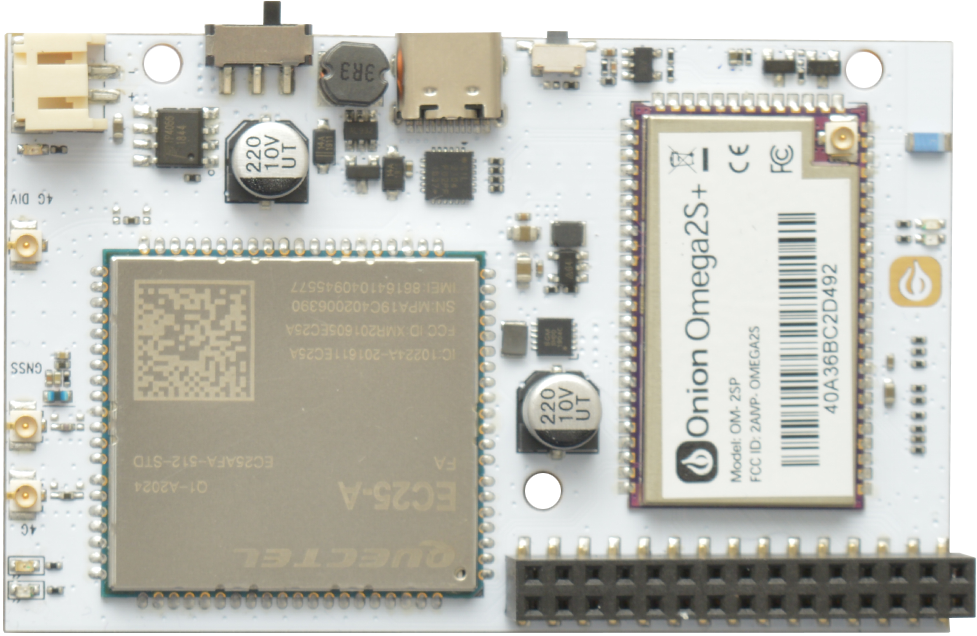
\includegraphics[width=0.2\textwidth]{figs/onion-omega.png}
    \caption{Onion Omega}
    \label{fig:onion-omega}
    \vspace{-1mm}
\end{wrapfigure}
Calculating drone-to-cloudlet latency is challenging since the Anafi, being a
commerical product that restricts modification of its onboard software,
functions as a black box. The inability to add software instrumentation on the
drone makes it difficult to determine when a given frame was transmitted from
the drone. To circumvent this restriction, Bala et al adapted the technique
George et al used for measuring motion-to-photon latency in augmented reality
\cite{george20}.


\begin{figure}[htbp]
\centerline{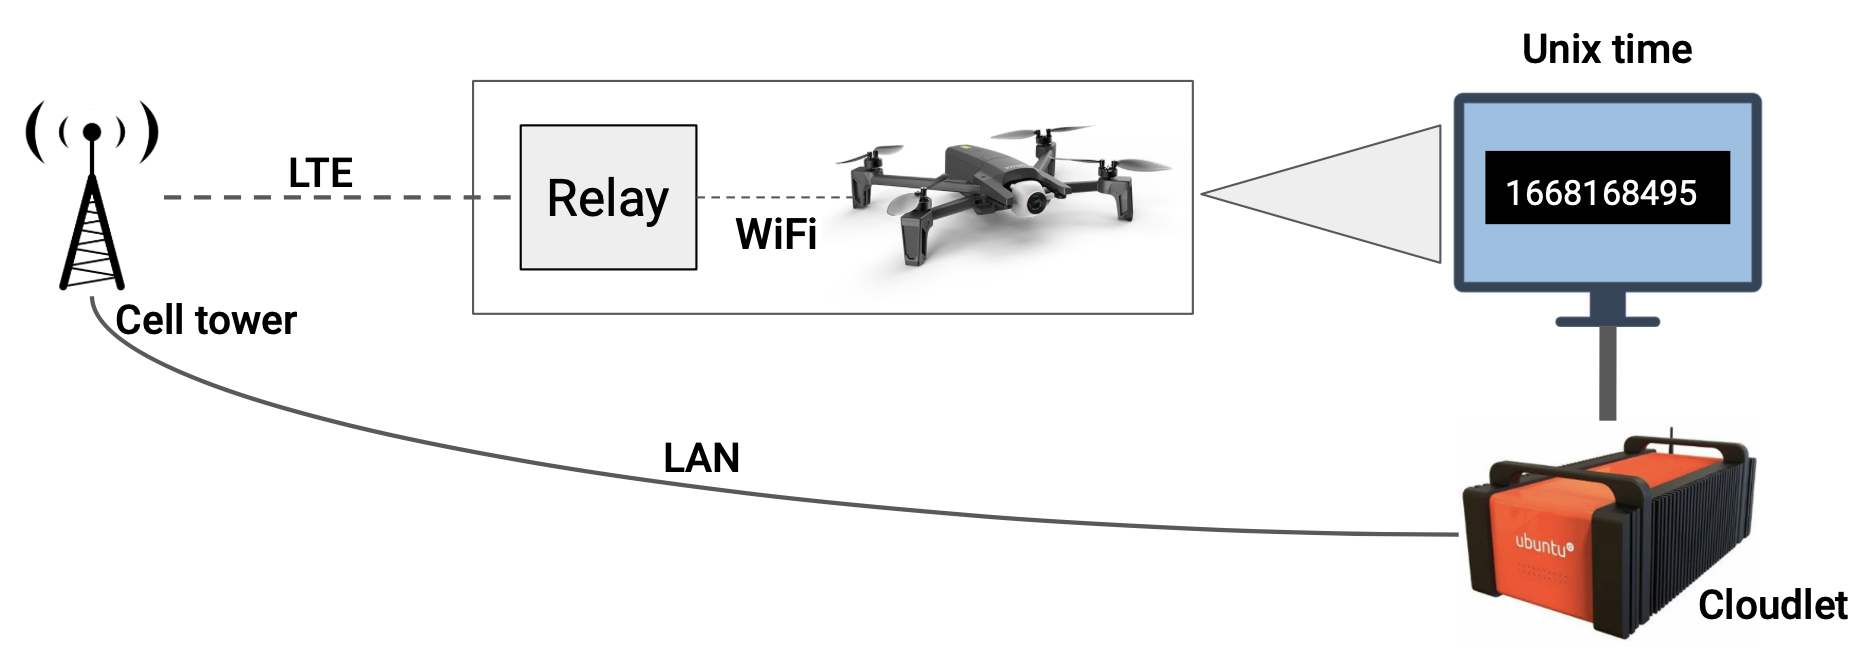
\includegraphics[width = .8\textwidth]{figs/mtp_pipeline.png}}
\caption{Technique for measuring end-to-end latency}
\label{fig:latency-measuring-technique}
\end{figure}
As shown in \cref{fig:latency-measuring-technique}, the drone is kept
stationary in a lab setting with its camera pointed at a display connected to
the cloudlet showing the current Unix timestamp at millisecond granularity. The
drone captures images containing the timestamp displayed and transmits them to
the cloudlet through the SteelEagle pipeline. The cloudlet records the
timestamp at which it receives each frame, storing the frame along with this
timestamp. To obtain the drone-to-cloudlet latency, these saved frames are
post-processed to compute the difference between the timestamps shown in each
frame and the timestamps at which they were received.

The mean latency of 933 ms reported by Bala et al is incredibly high.

\Cref{tab:latency_summary}

\begin{table}[htbp]
    \centering
    \caption{Drone-to-Cloudlet SteelEagle Latency (in ms)}
    \label{tab:latency_summary}
        \sisetup{
        detect-all,
        table-number-alignment = center,
        input-decimal-markers = {.},
        group-separator={,},
        group-minimum-digits=4
    }
    \begin{tabularx}{0.6\linewidth}{@{}
        X
        c%S[table-format=3.0]
        S[table-format=3.0]
        S[table-format=3.0]
        S[table-format=3.0]
        S[table-format=4.0]@{}
    }
    \toprule
    \textbf{Configuration} & \textbf{Average} & \textbf{Median} & \textbf{p95} & \textbf{Min} & \textbf{Max} \\
    \midrule
    \multicolumn{6}{@{}l}{\textbf{Cloudlet}} \\
    FFmpeg & 888 {\small $\pm$ 30} & 887 & 917 & 838 & 1030 \\
    PDrAW   & 380 {\small $\pm$ 15} & 379 & 402 & 344 & 420 \\
    %WiFi + FFmpeg & 841.52 & 841 & 868.3 & 16.79 & 807 & 879 \\
    %WiFi + PDrAW & 340.82 & 338.5 & 373.5 & 21.82 & 298 & 419 \\
    \midrule
    \multicolumn{6}{@{}l}{\textbf{AWS Small}} \\
    FFmpeg & 536 {\small $\pm$ 75} & 521 & 600 & 473 & 936 \\
    PDrAW   & 429 {\small $\pm$ 21} & 427 & 467 & 387 & 475 \\
    \midrule
    \multicolumn{6}{@{}l}{\textbf{AWS Big}} \\
    FFmpeg & 870 {\small $\pm$ 20} & 868 & 900 & 837 & 925 \\
    PDrAW   & 367 {\small $\pm$ 20} & 365 & 392 & 327 & 416 \\
    \bottomrule
    \end{tabularx}\\
    \vspace{0.1in}
    \footnotesize
    50 samples obtained for each configuration.
\end{table}

